\section{Problems}
%% TEMPLATE STUFF - WORK BELOW THIS BLOCK
%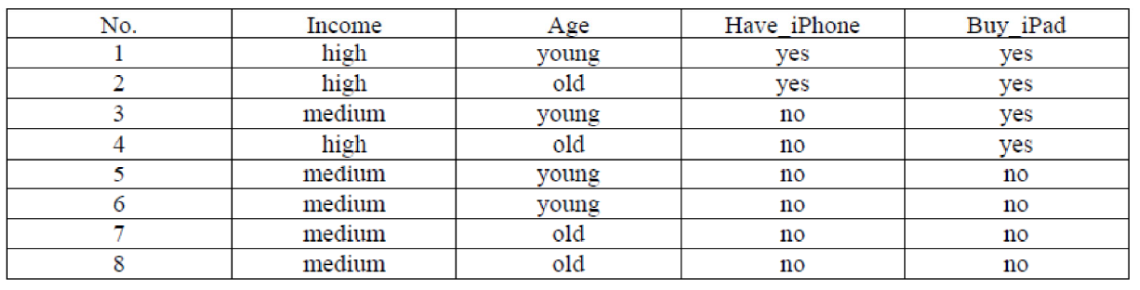
\includegraphics[width=1\textwidth]{media/hw5_q1.png}
%\begin{align}
%    P(I=m | iPad = y) &= \frac{1}{4} \label{eq:q1_1} \nonumber \\
%    P(I=m | iPad = n) &= \frac{4}{4} = 1
%\end{align}

\subsection{Question One}
\textbf{[logic neural network] [10 pts] You are given the following neural network which takes two binary valued inputs x1, x2, and the activation function is the threshold function (or indicator function, h(x) = 1 if x>0; or 0 otherwise). Which of the following logic function does it compute, OR, AND, Negative AND, or XOR? Please provide your argument (draw a truth table).}

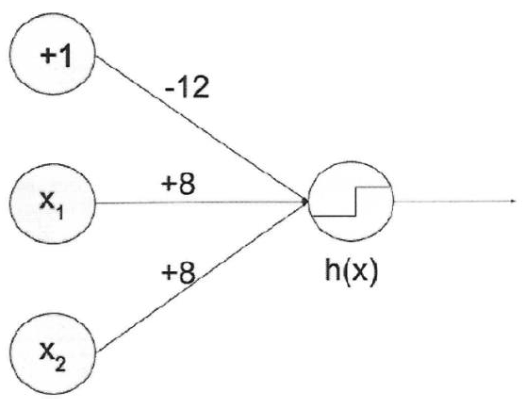
\includegraphics[width=0.5\textwidth]{media/hw7_q1.png}

We are given $h(x)$, which outputs the following:
\begin{align}
    z &= w \cdot x + b \label{eq:q1_1} \nonumber \\
    &= 1\cdot 12 + x_1 \cdot 8 + x_2 \cdot 8 \nonumber \\
    &= -12 + 8x_1 + 8x_2
\end{align}

Then according to the condition of $h(x)$, we obtain the following truth table for each potential value \{0, 1\} for $x_1$ and $x_2$:

\begin{table}[h!]
  \centering
  \begin{tabular}{|c|c|c|c|}
  \hline
  \(x_1\) & \(x_2\) & \(z\) & \(h(x)\) \\ \hline
  0       & 0       &  -12     &   0       \\ \hline
  0       & 1       &   -4    &    0      \\ \hline
  1       & 0       &   -4    &    0      \\ \hline
  1       & 1       &    4   &     1     \\ \hline
  \end{tabular}
  \end{table}

  Since the only time $h(x)=1$ is when both $x_1$ and $x_2$ are 1, this corresponds to the AND logic function.

\subsection{Question Two}

\textbf{[Forward and backward calculation] We have a function which takes a two-dimensional input $\mathbf{x} = (x_1, x_2)$ and has two parameters $\mathbf{w} = (w_1, w_2)$ given by:}

$$
f(\mathbf{x}; \mathbf{w}) = \sigma(\sigma(x_1 w_1) \cdot w_2 + x_2)
$$

\textbf{where}

$$
\sigma(x) = \frac{1}{1 + e^{-x}}.
$$

\textbf{We use backpropagation to estimate the right parameter values. We start by setting the parameters $w_1 = 1$, $w_2 = 2$. Assume that we are given a training point $x_1 = 1$, $x_2 = 0$, and $y = 5$.}

\textbf{(2a) [10 pts] Please calculate the prediction for the point $x_1 = 1$, $x_2 = 0$ given the current weight values of the model.}

\textbf{We can re-write the $f(\mathbf{x}; \mathbf{w})$ to}

$$
o_1 = \sigma(x_1 w_1)
$$
$$
o_2 = \sigma(o_1 w_2 + x_2)
$$

\textbf{and output $o_2$.}

Substituting the values, we get:

\begin{align}
  o_1 &= \sigma(x_1 w_1) \nonumber \\
      &= \sigma(1 \cdot 1) \nonumber \\
      &= \frac{1}{1 + e^{-1}} \nonumber \\
      &\approx 0.7311
\end{align}

\begin{align}
  o_2 &= \sigma(o_1 w_2 + x_2) \nonumber \\
      &= \sigma(0.7311 \cdot 2 + 0) \nonumber \\
      &= \sigma(1.4622) \nonumber \\
      &= \frac{1}{1 + e^{-1.4622}} \nonumber \\
      &\approx 0.8119
\end{align}

$\therefore o_2 \approx 0.8119$. 


\textbf{(2b) [10 pts] Please find the value of the gradient of the squared loss \( E(\mathbf{w}) = (y^* - y)^2 \) where \( y^* = o_2 \) is the output (or prediction) of the model.}

\textbf{Note that the gradient contains two entries}

\[
\left[ \frac{\partial E}{\partial w_1}, \frac{\partial E}{\partial w_2} \right].
\]


We start by first finding $\frac{\partial E}{\partial o_2}$:
\begin{align}
    \frac{\partial E}{\partial o_2} &= 2(o_2 - y) \nonumber \\
    &= 2(0.8119 - 5) \nonumber \\
    &= -8.3762
\end{align}

We then find $\frac{\partial E}{\partial w_2}$ using the chain rule:
\begin{align}
  \frac{\partial E}{\partial w_2} &= \frac{\partial E}{\partial o_2} \frac{\partial o_2}{\partial w_2} \label{eq:q2b_1}
\end{align}

We first find $\frac{\partial o_2}{\partial w_2}$:
\begin{align}
  \frac{\partial o_2}{\partial w_2} &= \sigma'(o_1 w_2 + x_2)\cdot o_1
\end{align}

where $\sigma'(z)=\sigma(z)(1-\sigma(z))$, and $z=o_1 w_2 + x_2 = 1.4622$. Then we have:
\begin{align}
  \frac{\partial o_2}{\partial w_2} &= \Bigg(\frac{1}{1+e^{-z}}\Big(1-\frac{1}{1+e^{-z}} \Big)\Bigg) \cdot o_1 \nonumber \\
  &= \Bigg(\frac{1}{1+e^{-1.4622}}\Big(1-\frac{1}{1+e^{-1.4622}} \Big)\Bigg) \cdot 0.8119 \nonumber \\
  &= 0.1240
\end{align}

Subbing this back into Eq. \ref{eq:q2b_1}:
\begin{align}
  \frac{\partial E}{\partial w_2} &= \frac{\partial E}{\partial o_2} \cdot \frac{\partial o_2}{\partial w_2} \nonumber \\
  &= -8.3762 \cdot 0.1240 \nonumber \\
  &= -1.0386
\end{align}


We now find the gradient with respect to $w_1$:
\begin{align}
    \frac{\partial o_2}{\partial o_1} &= w_2 (1 - o_2) o_2 \nonumber \\
    &= 2 \cdot (1 - 0.8119) \cdot 0.8119 \nonumber \\
    &\approx 0.3054
\end{align}

\begin{align}
    \frac{\partial o_1}{\partial w_1} &= x_1 (1 - o_1) o_1 \nonumber \\
    &= 1 \cdot (1 - 0.7311) \cdot 0.7311 \nonumber \\
    &\approx 0.1966
\end{align}

\begin{align}
    \frac{\partial E}{\partial w_1} &= \frac{\partial E}{\partial o_2} \cdot \frac{\partial o_2}{\partial o_1} \cdot \frac{\partial o_1}{\partial w_1} \nonumber \\
    &= -8.3762 \cdot 0.3054 \cdot 0.1966 \nonumber \\
    &\approx -0.5029
\end{align}

Therefore the final gradient with respect to $\mathbf{w}$ is:
\begin{align}
    \nabla_{\mathbf{w}} E &= \left[ \frac{\partial E}{\partial w_1}, \frac{\partial E}{\partial w_2} \right] \nonumber \\
    &= \left[ -0.5029, -1.0386 \right]
\end{align}


\subsection{Long Short-term Memory (LSTM) [20 pts]}

We are given two data points with 2 different timesteps. 

At the timestamp \( t = 1 \), we have data point \( (x_{1,1}, x_{1,2}, y_1) = (0.3, 0.6, 0.2) \). 

At the timestamp \( t = 2 \), we have data point \( (x_{2,1}, x_{2,2}, y_2) = (0.1, 1.0, 0.4) \). 

Here \( x_{t,1} \) and \( x_{t,2} \) are 2 input variables, \( y_t \) is the output variable, \( t \) is the time step.

Consider the traditional LSTM model. Initially, we have the following internal weight vectors and bias variables as follows:

\[
\mathbf{W}_f = \begin{pmatrix} 0.8 \\ 0.4 \\ 0.1 \end{pmatrix}, \quad \mathbf{b}_f = 0.2
\]
\[
\mathbf{W}_i = \begin{pmatrix} 0.9 \\ 0.8 \\ 0.7 \end{pmatrix}, \quad \mathbf{b}_i = 0.5
\]
\[
\mathbf{W}_a = \begin{pmatrix} 0.4 \\ 0.2 \\ 0.1 \end{pmatrix}, \quad \mathbf{b}_a = 0.3
\]
\[
\mathbf{W}_o = \begin{pmatrix} 0.6 \\ 0.4 \\ 0.1 \end{pmatrix}, \quad \mathbf{b}_o = 0.2
\]

In the model, we have the following gate variables. For each \( t = 1, 2, \dots \):
\begin{itemize}
    \item Forget gate variable (weight) \( f_t \);
    \item Input gate variable (weight) \( i_t \);
    \item Candidate cell state \( \tilde{C}_t \);
    \item Cell state variable \( C_t \);
    \item Output gate variable \( o_t \);
    \item Final output variable \( \tilde{y}_t \) (this may have a different notation from our lecture slides).
\end{itemize}

Suppose that \( y_0 = s_0 = 0 \) and \( C_0 = 0 \).

Consider the input forward propagation step only.

\subsubsection*{(3.a) [10 pts]} \textbf{What are the values of the above gate variables (1 – 6) when \( t = 1 \) and when \( t = 2 \)? Please show each answer up to 4 decimal places.}

\subsubsection*{(3.a) [10 pts] Answer}

We compute the values of the gate variables for each timestep \( t = 1 \) and \( t = 2 \). The formulae for the gate variables are:

\begin{align}
    f_t &= \sigma(\mathbf{W}_f^\top \mathbf{x}_t + \mathbf{b}_f) \nonumber \\
    i_t &= \sigma(\mathbf{W}_i^\top \mathbf{x}_t + \mathbf{b}_i) \nonumber \\
    \tilde{C}_t &= \tanh(\mathbf{W}_a^\top \mathbf{x}_t + \mathbf{b}_a) \nonumber \\
    C_t &= f_t \cdot C_{t-1} + i_t \cdot \tilde{C}_t \nonumber \\
    o_t &= \sigma(\mathbf{W}_o^\top \mathbf{x}_t + \mathbf{b}_o) \nonumber \\
    \tilde{y}_t &= o_t \cdot \tanh(C_t)\nonumber 
\end{align}

For the first timestep \( t = 1 \), we have:
\begin{align}
    f_1 &= \sigma(0.8 \cdot 0.3 + 0.4 \cdot 0.6 + 0.1 \cdot 0 + 0.2) \nonumber \\
        &= \sigma(0.24 + 0.24 + 0 + 0.2) \nonumber \\
        &= \sigma(0.68) \nonumber \\
        &= 0.6637
\end{align}
\begin{align}
    i_1 &= \sigma(0.9 \cdot 0.3 + 0.8 \cdot 0.6 + 0.7 \cdot 0 + 0.5) \nonumber \\
        &= \sigma(0.27 + 0.48 + 0 + 0.5) \nonumber \\
        &= \sigma(1.25) \nonumber \\
        &= 0.7773
\end{align}
\begin{align}
    \tilde{C}_1 &= \tanh(0.4 \cdot 0.3 + 0.2 \cdot 0.6 + 0.1 \cdot 0 + 0.3) \nonumber \\
                &= \tanh(0.12 + 0.12 + 0 + 0.3) \nonumber \\
                &= \tanh(0.54) \nonumber \\
                &= 0.4930
\end{align}
\begin{align}
    C_1 &= f_1 \cdot C_0 + i_1 \cdot \tilde{C}_1 \nonumber \\
        &= 0.6637 \cdot 0 + 0.7773 \cdot 0.4930 \nonumber \\
        &= 0.3831
\end{align}
\begin{align}
    o_1 &= \sigma(0.6 \cdot 0.3 + 0.4 \cdot 0.6 + 0.1 \cdot 0 + 0.2) \nonumber \\
        &= \sigma(0.18 + 0.24 + 0 + 0.2) \nonumber \\
        &= \sigma(0.62) \nonumber \\
        &= 0.6508
\end{align}
\begin{align}
    \tilde{y}_1 &= o_1 \cdot \tanh(C_1) \nonumber \\
                &= 0.6508 \cdot \tanh(0.3831) \nonumber \\
                &= 0.6508 \cdot 0.3651 \nonumber \\
                &= 0.2377
\end{align}

For the second timestep \( t = 2 \), we have:
\begin{align}
    f_2 &= \sigma(0.8 \cdot 0.1 + 0.4 \cdot 1.0 + 0.1 \cdot 0 + 0.2) \nonumber \\
        &= \sigma(0.08 + 0.4 + 0 + 0.2) \nonumber \\
        &= \sigma(0.68) \nonumber \\
        &= 0.6637
\end{align}
\begin{align}
    i_2 &= \sigma(0.9 \cdot 0.1 + 0.8 \cdot 1.0 + 0.7 \cdot 0 + 0.5) \nonumber \\
        &= \sigma(0.09 + 0.8 + 0 + 0.5) \nonumber \\
        &= \sigma(1.39) \nonumber \\
        &= 0.8006
\end{align}
\begin{align}
    \tilde{C}_2 &= \tanh(0.4 \cdot 0.1 + 0.2 \cdot 1.0 + 0.1 \cdot 0 + 0.3) \nonumber \\
                &= \tanh(0.04 + 0.2 + 0 + 0.3) \nonumber \\
                &= \tanh(0.54) \nonumber \\
                &= 0.4930
\end{align}
\begin{align}
    C_2 &= f_2 \cdot C_1 + i_2 \cdot \tilde{C}_2 \nonumber \\
        &= 0.6637 \cdot 0.3831 + 0.8006 \cdot 0.4930 \nonumber \\
        &= 0.2542 + 0.3945 \nonumber \\
        &= 0.6487
\end{align}
\begin{align}
    o_2 &= \sigma(0.6 \cdot 0.1 + 0.4 \cdot 1.0 + 0.1 \cdot 0 + 0.2) \nonumber \\
        &= \sigma(0.06 + 0.4 + 0 + 0.2) \nonumber \\
        &= \sigma(0.66) \nonumber \\
        &= 0.6590
\end{align}
\begin{align}
    \tilde{y}_2 &= o_2 \cdot \tanh(C_2) \nonumber \\
                &= 0.6590 \cdot \tanh(0.6487) \nonumber \\
                &= 0.6590 \cdot 0.5713 \nonumber \\
                &= 0.3765
\end{align}


\subsubsection*{(3.b) [10 pts]} \textbf{What are the error values (in terms of absolute error between true value \( y_t \) and prediction \( \tilde{y}_t \)) of the final output variables when \( t = 1 \) and \( t = 2 \)? Please show each answer up to 4 decimal places.}

For each time step \( t \), we have the absolute errors:

\begin{align}
    \text{Error at } t = 1 &= \left| y_1 - \tilde{y}_1 \right| \nonumber \\
    &= \left| 0.2 - 0.2377 \right| \nonumber \\
    &= 0.0377
\end{align}

\begin{align}
    \text{Error at } t = 2 &= \left| y_2 - \tilde{y}_2 \right| \nonumber \\
    &= \left| 0.4 - 0.3765 \right| \nonumber \\
    &= 0.0235
\end{align}